\documentclass[final,hyperref={pdfpagelabels=false}]{beamer}
\usepackage{grffile}
\mode<presentation>{\usetheme{I6pd2}}
\usepackage[english]{babel}
%\usepackage{natbib}
\usepackage[latin1]{inputenc}
\usepackage{amsmath,amsthm, amssymb, latexsym}
\boldmath
\usepackage[orientation=landscape,size=a0,scale=1.1,debug]{beamerposter}
\usepackage{array,booktabs,tabularx}
\newcolumntype{Z}{>{\centering\arraybackslash}X}
\newcommand{\pphantom}{\textcolor{ta3aluminium}}

\listfiles

\setbeamertemplate{bibliography item}{\insertbiblabel}
\setbeamercolor{bibliography item}{fg=white}
\setbeamercolor*{bibliography entry author}{fg=white}
\setbeamercolor*{bibliography entry title}{fg=white} 
\setbeamercolor*{bibliography entry location}{fg=white} 
\setbeamercolor*{bibliography entry note}{fg=white}  

 
\title{\LARGE Big Data Analytics Pipeline for the Analysis of TESS Full Frame Images}
\author{Matthew Wampler-Doty \& Dr. John Doty}
\institute[Noqsi Aerospace]{Noqsi Aerospace, Ltd. \& MIT}
\date[]{}
\newlength{\columnheight}
\setlength{\columnheight}{105cm}

\begin{document}
\begin{frame}
  \begin{columns}
    \begin{column}{.49\textwidth}
      \begin{beamercolorbox}[center,wd=\textwidth]{postercolumn}
        \begin{minipage}[T]{.95\textwidth}  % tweaks the width, makes a new \textwidth
          \parbox[t][\columnheight]{\textwidth}{
            \begin{block}{Introduction}
	    The goals of this research are:
            \begin{columns}
	            \begin{column}{.70\textwidth}
		              \begin{itemize}
		              \item Create a \emph{fast, high fidelity} simulation of the TESS Full Frame Images (FFIs)
		              \item Develop a data processing system that takes the TESS FFIs and looks for items such as:
		              \begin{itemize}
		              	\item Tidal disruption events
			        \item Gamma-ray burst afterglow
				\item Low surface brightness structures
				\item Unusual variable objects
				\item Exoplanets around non-targeted stars
		              \end{itemize}
		              \end{itemize}
		     \end{column}
		     \begin{column}{.28\textwidth}
		     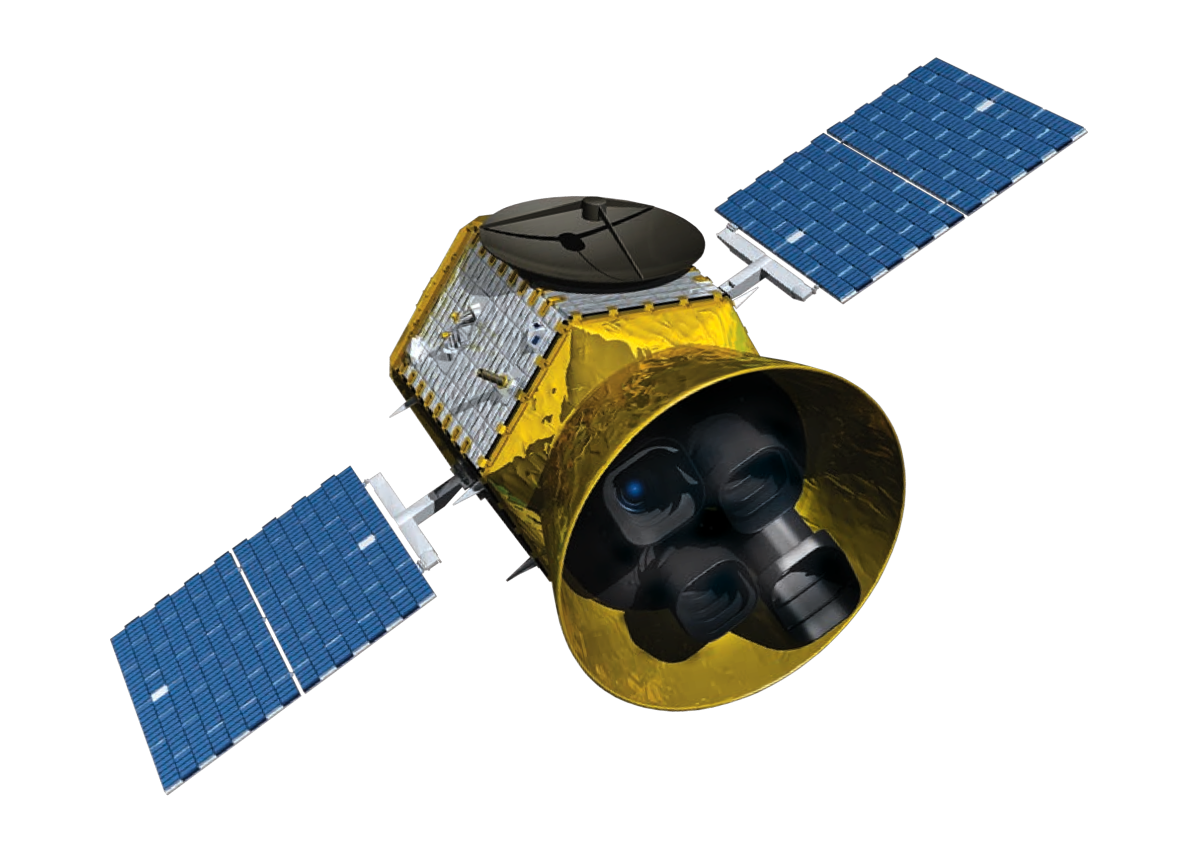
\includegraphics[width=0.80\linewidth]{figures/TESS.png}
		     \end{column}         
              \end{columns}
            \end{block}

            \vspace{2cm}
            \begin{block}{Conventional Data Processing Pipeline}
            \begin{itemize}
              	\item Conventional processing for astronomical data attempts to scrub out artifacts and then extract results from clean images.
		\item Computational requirements are relatively low, but the scrubbing process may remove real effects and makes error estimates less accurate.
		\item In the past, this approach was necessary due to the high expense of computation.
	    \end{itemize}
	      \begin{center}
              
\includegraphics[width=0.75\linewidth]{figures/Conventional_Pipeline.pdf}
              \end{center}
            \end{block}

            \vspace{2cm}
            \begin{block}{Our Simulation-Driven Processing Loop}
            \begin{itemize}
            \item  In theory, running a model through a simulation to compare with the rawest data available is statistically more robust.
            \item In order get good agreement, we must put every significant effect in the model including artifacts conventionally removed.
            \item It will be harder to ignore unexpected events and phenomena.
            \item Running multiple simulations is computationally expensive, but the cost of Gflop/s cores is $\approx\$0.20$ per core and falling rapidly.
            \end{itemize}
              \begin{center}
              
\includegraphics[width=0.75\linewidth]{figures/Our_Pipeline.pdf}
              \end{center}
            \end{block}
            \begin{block}{Project Plan}
            \begin{itemize}
		\item Primarily a software project
		\item Small team, open source, highest productivity 21st century methodology
		\item Outside contributions are welcome
		\item Database of results freely accessible
		\item Give URL of GitHub project here
	    \end{itemize}
	    \vspace{1cm}
The authors acknowledge productive discussions with Garrett Jernigan, Roland Vanderspek, and George Ricker.
            \end{block}
          }
        \end{minipage}
      \end{beamercolorbox}
    \end{column}
    % ---------------------------------------------------------%
    % end the column

    % ---------------------------------------------------------%
    % Set up a column 
    \begin{column}{.49\textwidth}
      \begin{beamercolorbox}[center,wd=\textwidth]{postercolumn}
        \begin{minipage}[T]{.95\textwidth}
          \parbox[t][\columnheight]{\textwidth}{
            \begin{block}{Simulated TESS Full Frame Image}
            Image generated by Zach Berta-Thompson using his existing simulator
              \begin{columns}
                \begin{column}{.70\textwidth}
                \begin{itemize}
                    \item In our new proposed simulator, the \emph{Sky Model} will include catalog stars, galaxies, solar system bodies, diffuse galactic light, zodiacal light, ...
                    \vfill
                    \item We will simulate optics, CCD detector physics, and electronics.
                    \begin{itemize}
                    	\item Every photon from every star is independent, so we can rapidly generate images using many processor cores in parallel. We will employ \texttt{CUDA}, (Compute Unified Device Architecture), and possibly other technologies. 
			\item We can accelerate these calculations by choosing a representative sample of photon paths and weighting, yielding a more accurate estimate of the expectation value than a straight Monte Carlo simulation.
                    \end{itemize}
                    \vfill
                    \item We will also simulate TESS on-board data processing, including the cosmic ray scrubbing, since that is part of the raw image capture process.
                    \vfill
                \end{itemize}
                \end{column}
                \begin{column}{.28\textwidth}
                  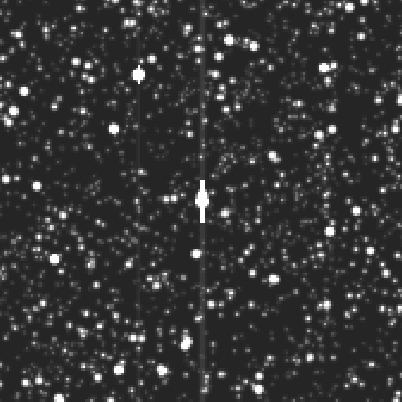
\includegraphics[width=0.80\linewidth]{figures/ffi_simulation.jpg}
		\end{column}
	       \end{columns}
            \end{block}
            \vspace{1cm}
            \begin{block}{Science}
            	\begin{columns}
	                	\begin{column}{.70\textwidth}
		            	\begin{itemize}
					\item Series of images give rise to time series that we can mine looking for various objects and events.
					\item To evaluate the performance of a particular data mining algorithm, we will simulate artificial data. We may use our simulator or another.
					\item We intend to bring in statistical processing and evaluation methods from as many sources as practical (machine vision, economics, ...).
					\item We will compare algorithms using various statistical performance measurements, such as $F_1$ scores, area under ROC Curve (see figure to the right) and others.
					$$ F_1 = 2 \cdot \frac{\textup{precision} \cdot \textup{recall}}{\textup{precision} + \textup{recall}} $$
					\item We may be able to find interesting objects by applying statistical methods from complex systems theory. We expect that objects with unusual measures of variability will prove to be unusual physically.
					\begin{itemize}
						\item \emph{Hurst exponents} \cite{hurst_longterm_1951}
						\begin{itemize}
							\item A measure of long term time dependence
							\item Applications in civil engineering and finance
							\item Defined as a quantity $H$ where
							$$\mathbb{E} \left[\frac{R(n)}{S(n)}\right] = C n^H \textup{ as }n \to \infty$$
%							where
%							\begin{itemize}
%								\item $R(n)$ is the range of the first $n$ values in the time series
%								\item $S(n)$ is the standard deviation
%								\item $E[X]$ is the expected value of $X$
%								\item $n$ is the timespan of the observation
%								\item $C$ is a constant
%							\end{itemize}
						\end{itemize}
						\item \emph{Tail $\alpha$-value}
						\begin{itemize}
							\item Objects with little extreme variation, like the Gaussian, are dubbed \emph{thin tailed}.
							\item Objects with wild variation, like the object recently found by Boyajian et. al \cite{boyajian_planet_2015}, are dubbed \emph{fat tailed}.
							\item There are an number of estimators we may use. One estimator due to Taleb \cite{taleb_silent_2015} employs the fact that for fat tailed distributions with a tail coefficient $\alpha > 2$, then
							$$ \Xi[X] = \frac{\sqrt{\mathbb{E}[X^2]}}{\mathbb{E}[|X|]} = \frac{\sqrt{\pi}\sqrt{\frac{\alpha}{\alpha -2}}\Gamma\left(\frac{\alpha}{2}\right)}{\sqrt{\alpha} \Gamma \left(\frac{\alpha - 1}{2} \right)}$$
							So $\alpha$ can be estimated by computing $\Xi^{-1}\left[\frac{\sqrt{\mathbb{E}[X^2]}}{\mathbb{E}[|X|]}\right]$
						\end{itemize}
					\end{itemize}
		                \end{itemize}
	                \end{column}
	                \begin{column}{.28\textwidth}
	                         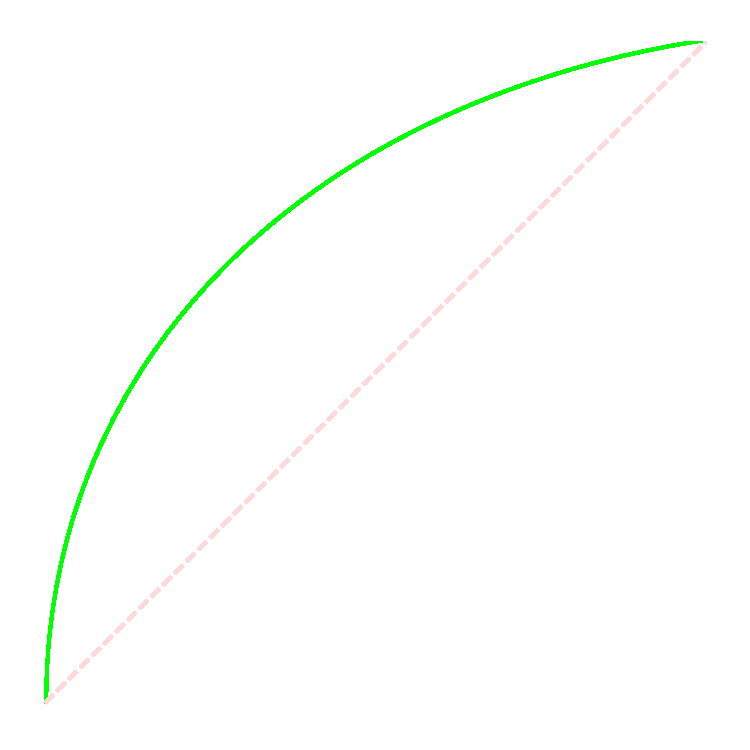
\includegraphics[width=0.80\linewidth]{figures/ROC}
	       		\end{column}
		\end{columns}
            \end{block}
            \begin{block}{Bibliography}
            \small
	   \bibliographystyle{plain}
            \bibliography{./bibliography.bib}
            \end{block}
          }

        \end{minipage}
      \end{beamercolorbox}
    \end{column}
    % ---------------------------------------------------------%
    % end the column
  \end{columns}
  \vskip1ex
  \tiny\hfill{Created with \LaTeX \texttt{beamerposter}  \url{http://www-i6.informatik.rwth-aachen.de/~dreuw/latexbeamerposter.php} \hskip1em}
\end{frame}


\end{document}

%%%%%%%%%%%%%%%%%%%%%%%%%%%%%%%%%%%%%%%%%%%%%%%%%%%%%%%%%%%%%%%%%%%%%%%%%%%%%%%%%%%%%%%%%%%%%%%%%%%
%%% Local Variables: 
%%% mode: latex
%%% TeX-PDF-mode: t
%%% End:
